%%%%%%%%%%%%%%%%%%%%%%%%%%%%%%%%%%%%

\section{Confidence intervals}

%%%%%%%%%%%%%%%%%%%%%%%%%%%%%%%%%%%%

\subsection{Why do we report confidence intervals?}

%%%%%%%%%%%%%%%%%%%%%%%%%%%%%%%%%%%%

\begin{frame}[shrink]
\frametitle{Confidence intervals}

\begin{itemize}

\item A plausible range of values for the population parameter is called a \hl{confidence interval}.

\item Using only a sample statistic to estimate a parameter is like fishing in a murky lake with a spear, and using a confidence interval is like fishing with a net.
$\:$ \\
$\:$ \\
\begin{columns}[c]
\column{0.25\textwidth}

\includegraphics[width=\textwidth]{4-2_conf_int/figures/spear}
\column{0.5\textwidth}
{\small
We can throw a spear where we saw a fish but we will probably miss. If we toss a net in that area, we have a good chance of catching the fish.
}
\column{0.25\textwidth}

\includegraphics[width=\textwidth]{4-2_conf_int/figures/net}
\end{columns}
$\:$ \\
\item If we report a point estimate, we probably won't hit the exact population parameter. If we report a range of plausible values we have a good shot at capturing the parameter. 

\end{itemize}

{\tiny Photos by Mark Fischer (http://www.flickr.com/photos/fischerfotos/7439791462) and Chris Penny (http://www.flickr.com/photos/clearlydived/7029109617) on Flickr.}

% spear fig: http://www.flickr.com/photos/clearlydived/7029109617/sizes/q/
% net fig: http://www.flickr.com/photos/fischerfotos/7439791462/sizes/q/

\end{frame}

%%%%%%%%%%%%%%%%%%%%%%%%%%%%%%%%%%%%

\subsection{Constructing a confidence interval}

%%%%%%%%%%%%%%%%%%%%%%%%%%%%%%%%%%%%

\begin{frame}
\frametitle{Average number of exclusive relationships}

\dq{A random sample of 50 college students were asked how many exclusive relationships they have been in so far. This sample yielded a mean of 3.2 and a standard deviation of 1.74. Estimate the true average number of exclusive relationships using this sample.}

\pause 

\vspace{-0.5cm}
\[ \bar{x} = 3.2 \qquad s = 1.74 \]

\pause

The approximate 95\% confidence interval is defined as 
\[ point~estimate \pm 2 \times SE \]

\pause

\vspace{-0.25cm}
\[ SE = \frac{s}{\sqrt{n}} = \frac{1.74}{\sqrt{50}} \approx 0.25 \]

\pause

\vspace{-0.25cm}
\begin{eqnarray*}
\bar{x} \pm 2 \times SE &=& 3.2 \pm 2 \times 0.25 \\
\pause
&=& (3.2 - 0.5, 3.2 + 0.5) \\
\pause
&=& (2.7, 3.7)
\end{eqnarray*}


\end{frame}

%%%%%%%%%%%%%%%%%%%%%%%%%%%%%%%%%%%

\begin{frame}
\frametitle{}

\pq{Which of the following is the correct interpretation of this confidence interval?}

We are 95\% confident that
\begin{enumerate}[(a)]
\item the average number of exclusive relationships college students in this sample have been in is between 2.7 and 3.7.
\solnMult{college students on average have been in between 2.7 and 3.7 exclusive relationships.}
\item a randomly chosen college student has been in 2.7 to 3.7 exclusive relationships.
\item 95\% of college students have been in 2.7 to 3.7 exclusive relationships.
\end{enumerate}

\end{frame}

%%%%%%%%%%%%%%%%%%%%%%%%%%%%%%%%%%%

\subsection{A more accurate interval}

%%%%%%%%%%%%%%%%%%%%%%%%%%%%%%%%%%%

\begin{frame}
\frametitle{A more accurate interval}

\formula{Confidence interval, a general formula}
{\[ point~estimate\pm z^\star \times SE \] }

\pause

Conditions when the point estimate = $\bar{x}$:
\begin{enumerate}

\item \hlGr{Independence:} Observations in the sample must be independent
\begin{itemize}
\item random sample/assignment
\item if sampling without replacement, $n <$ 10\% of population
\end{itemize}

\item \hlGr{Sample size / skew:} $n \ge 30$ and population distribution should not be extremely skewed

\end{enumerate}

$\:$ \\
\pause

\orange{Note:} We will discuss working with samples where $n < 30$ in the next chapter.

\end{frame}

%%%%%%%%%%%%%%%%%%%%%%%%%%%%%%%%%%%%

\subsection{Capturing the population parameter}

%%%%%%%%%%%%%%%%%%%%%%%%%%%%%%%%%%%

\begin{frame}
\frametitle{What does 95\% confident mean?}

\begin{itemize}

\item Suppose we took many samples and built a confidence interval from each sample using the equation $point~estimate \pm 2 \times SE$.

\item Then about 95\% of those intervals would contain the true population mean ($\mu$). 

\end{itemize}

\twocol{0.5}{0.5}
{
\begin{itemize}

\item The figure shows this process with 25 samples, where 24 of the resulting confidence intervals contain the true average number of exclusive relationships, and one does not.

\end{itemize}
}
{
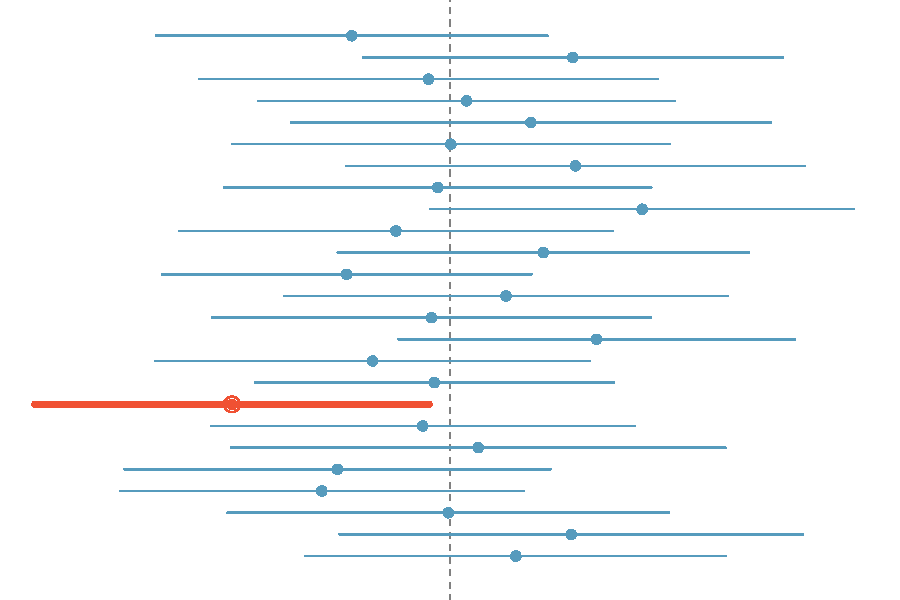
\includegraphics[width=\textwidth]{4-2_conf_int/figures/95PercentConfidenceInterval/95PercentConfidenceInterval}
}

\end{frame}

%%%%%%%%%%%%%%%%%%%%%%%%%%%%%%%%%%%

\begin{frame}
\frametitle{Width of an interval}

\dq{If we want to be more certain that we capture the population parameter, i.e. increase our confidence level, should we use a wider interval or a smaller interval?}

\pause

\soln{A wider interval.}

$\:$ \\

\pause

\dq{Can you see any drawbacks to using a wider interval?}
\begin{center}

\includegraphics[width=0.9\textwidth]{4-2_conf_int/figures/garfield}
\end{center}

\pause

\soln{If the interval is too wide it may not be very informative.}

\end{frame}

{\scriptsize Image source: http://web.as.uky.edu/statistics/users/earo227/misc/garfield\_weather.gif}

%%%%%%%%%%%%%%%%%%%%%%%%%%%%%%%%%%%

\subsection{Changing the confidence level}

%%%%%%%%%%%%%%%%%%%%%%%%%%%%%%%%%%%

\begin{frame}
\frametitle{Changing the confidence level}

\[ point~estimate\pm z^\star \times SE \] 

\begin{itemize}

\item In a confidence interval, $z^\star \times SE$ is called the \hl{margin of error}, and for a given sample, the margin of error changes as the confidence level changes.

\item In order to change the confidence level we need to adjust $z^\star$ in the above formula.

\item Commonly used confidence levels in practice are 90\%, 95\%, 98\%, and 99\%.

\item For a 95\% confidence interval, $z^\star = 1.96$.

\item However, using the standard normal ($z$) distribution, it is possible to find the appropriate $z^\star$ for any confidence level.

\end{itemize}

\end{frame}

%%%%%%%%%%%%%%%%%%%%%%%%%%%%%%%%%%%%

\begin{frame}

\pq{Which of the below Z scores is the appropriate $z^\star$ when calculating a 98\% confidence interval?}

\begin{multicols}{2}
\begin{enumerate}[(a)]
\item $Z = 2.05$
\item $Z = 1.96$
\solnMult{$Z = 2.33$}
\item $Z = -2.33$
\item $Z = -1.65$
\item[]
\end{enumerate}
\end{multicols}

\soln{\only<2>{
\begin{center}
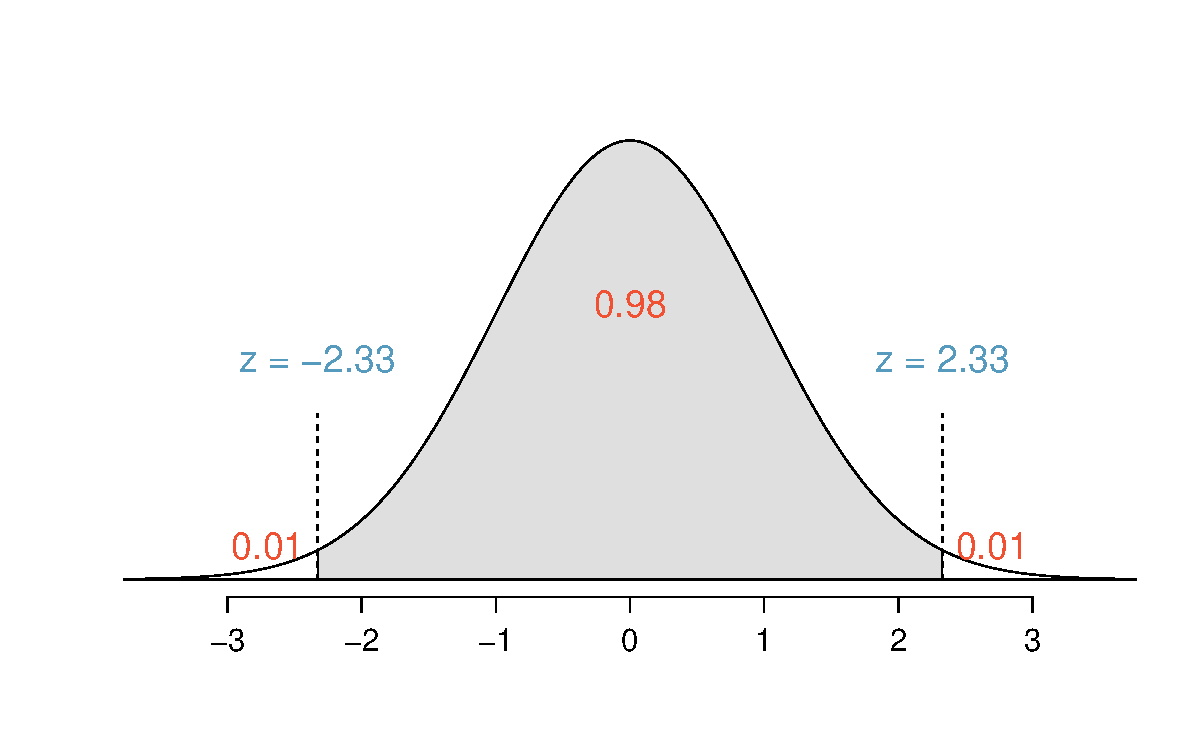
\includegraphics[width=0.7\textwidth]{4-2_conf_int/figures/middle98/middle98}
\end{center}
}}

\end{frame}

%%%%%%%%%%%%%%%%%%%%%%%%%%%%%%%%%%%
